%!TEX program = xelatex
\documentclass[aspectratio=169, 10pt]{beamer}

% --- Codificação e Idioma ---
\usepackage{polyglossia}
\setdefaultlanguage{brazil}
\usepackage{fontspec}
\defaultfontfeatures{Ligatures=TeX}

% --- Pacotes Matemáticos e Tabelas ---
\usepackage{amsmath, amssymb}
\usepackage{booktabs}
\usepackage{colortbl}
\usepackage{array}
\usepackage{tabularx}
\usepackage{graphicx}
\usepackage{tikz}
\usetikzlibrary{arrows.meta, positioning, shapes.geometric, calc}

% --- Paleta de Cores (Poli-USP / Corporativo) ---
\definecolor{NavyDark}{HTML}{0B2545}
\definecolor{PoliBlue}{HTML}{134074}
\definecolor{AccentTeal}{HTML}{1B998B}
\definecolor{AlertCoral}{HTML}{C83E4D}
\definecolor{WarnAmber}{HTML}{D9822B}
\definecolor{SoftBg}{HTML}{F4F6F9}
\definecolor{BorderGray}{HTML}{D6DCE5}
\definecolor{TextDark}{HTML}{222831}
\definecolor{TextMuted}{HTML}{5C677D}

% --- Configuração do Tema Beamer ---
\usetheme{default}
\usecolortheme{default}
\setbeamertemplate{navigation symbols}{}

\setbeamercolor{normal text}{fg=TextDark, bg=white}
\setbeamercolor{structure}{fg=PoliBlue}
\setbeamercolor{frametitle}{fg=NavyDark, bg=white}
\setbeamercolor{title}{fg=white}
\setbeamercolor{subtitle}{fg=SoftBg}
\setbeamercolor{author}{fg=SoftBg}
\setbeamercolor{institute}{fg=SoftBg}
\setbeamercolor{item}{fg=PoliBlue}
\setbeamercolor{block title}{fg=white, bg=PoliBlue}
\setbeamercolor{block body}{fg=TextDark, bg=SoftBg}

% --- Cabeçalho dos Slides ---
\setbeamertemplate{frametitle}{%
  \vspace{0.25cm}
  \begin{beamercolorbox}[wd=\paperwidth, leftskip=0.6cm, rightskip=0.6cm]{frametitle}
    \usebeamerfont{frametitle}\textbf{\insertframetitle}%
    \ifx\insertframesubtitle\@empty\else
      \\[0.06cm]{\small\color{TextMuted}\insertframesubtitle}%
    \fi
  \end{beamercolorbox}
  \vspace{0.08cm}
  \noindent{\color{PoliBlue}\rule{\textwidth}{1.2pt}}
  \vspace{0.1cm}
}

% --- Rodapé dos Slides ---
\setbeamertemplate{footline}{%
  \ifnum\theframenumber>1
    \begin{tikzpicture}[remember picture, overlay]
      \draw[BorderGray, line width=0.6pt] ($(current page.south west)+(0.6cm,0.5cm)$) -- ($(current page.south east)+(-0.6cm,0.5cm)$);
      \node[anchor=west, font=\scriptsize\color{TextMuted}] at ($(current page.south west)+(0.6cm,0.28cm)$) {PTC3567 -- Previsão de Churn no Varejo (VAI Store) \textbar{} \insertsectionhead};
      \node[anchor=east, font=\scriptsize\bfseries\color{PoliBlue}] at ($(current page.south east)+(-0.6cm,0.28cm)$) {\insertframenumber\ / \inserttotalframenumber};
    \end{tikzpicture}
  \fi
}

% --- Caixas Customizadas ---
\newcommand{\card}[3][PoliBlue]{%
  \noindent\begin{tikzpicture}
    \node[draw=BorderGray, fill=SoftBg, rounded corners=4pt, inner sep=7pt, text width=\dimexpr#2-14.8pt\relax, align=left] (box) {#3};
    \fill[#1] (box.north west) rectangle ([xshift=3.5pt]box.south west);
  \end{tikzpicture}%
}

\newcommand{\kpicard}[3][PoliBlue]{%
  \noindent\begin{tikzpicture}
    \node[draw=BorderGray, fill=SoftBg, rounded corners=4pt, inner sep=6pt, minimum width=\dimexpr#2-1pt\relax, align=center] (box) {%
      {\LARGE\bfseries\color{#1}#3}%
    };
  \end{tikzpicture}%
}

\begin{document}

% ==============================================================================
% SLIDE 1: CAPA
% ==============================================================================
\begin{frame}[plain]
  \begin{tikzpicture}[remember picture, overlay]
    \fill[NavyDark] (current page.north west) rectangle ([xshift=11.0cm]current page.south west);
    \fill[AccentTeal] ([xshift=11.0cm]current page.north west) rectangle ([xshift=11.18cm]current page.south west);
    \fill[SoftBg] ([xshift=11.18cm]current page.north west) rectangle (current page.south east);

    \node[anchor=west, text width=9.6cm, align=left] at ($(current page.west)+(0.8cm, 0.5cm)$) {%
      {\footnotesize\color{AccentTeal}\textbf{APRESENTAÇÃO FINAL DE PROJETO}}\\[0.35cm]
      {\LARGE\bfseries\color{white} Previsão de \textit{Churn} de Clientes no Varejo (VAI Store)}\\[0.45cm]
      {\small\color{SoftBg} PTC3567 -- Ciência de Dados em Automação e Engenharia (Poli-USP)}\\[0.8cm]
      {\footnotesize\color{BorderGray}\textbf{Autores:}}\\
      {\small\color{white} Mariana Aquino Rocha}\\
      {\small\color{white} Lucas Parisotto Fabre}\\
      {\small\color{white} Roberto Machado e Silva Gomide}
    };

    \node[anchor=center] at ($(current page.east)+(-2.4cm, 0.2cm)$) {%
      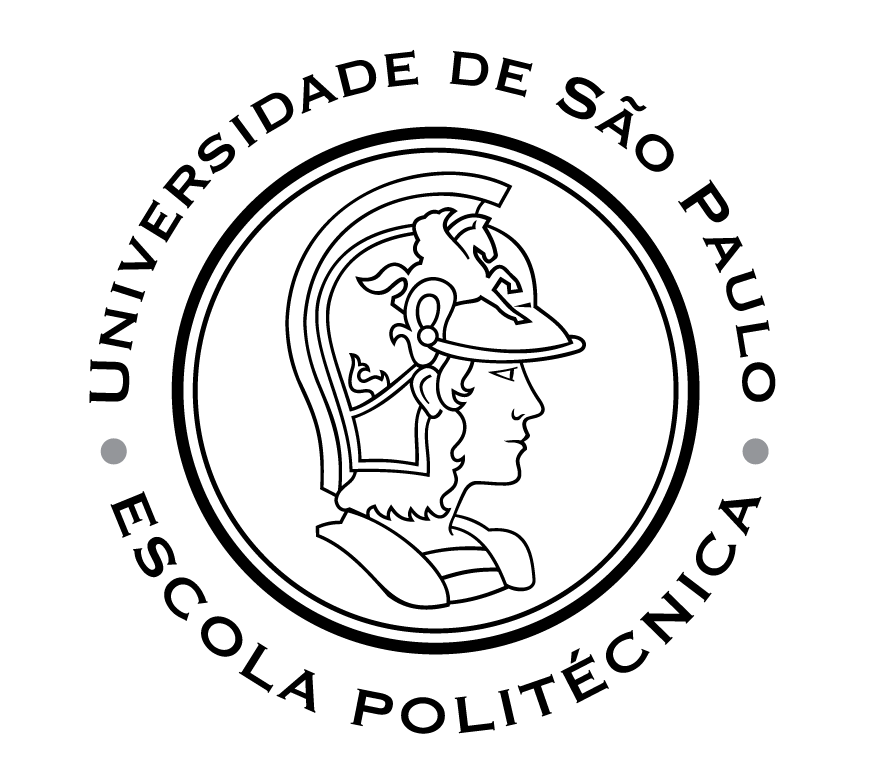
\includegraphics[width=3.5cm]{../latex/imagens/Poli.png}%
    };
  \end{tikzpicture}
\end{frame}

% ==============================================================================
% SEÇÃO 1: INTRODUÇÃO E PROBLEMA DE NEGÓCIO
% ==============================================================================
\section{1. Introdução e Problema}

% SLIDE 2: O Problema do Churn Silencioso
\begin{frame}{O Problema do \textit{Churn} Silencioso}
  \framesubtitle{Contexto de negócio e escopo da base VAI Store / Visagio (2024)}
  \begin{columns}[c]
    \begin{column}{0.48\textwidth}
      \card[AlertCoral]{\linewidth}{%
        \scriptsize\textbf{\color{AlertCoral}Desafio:} No varejo físico não há cancelamento formal — o cliente apenas deixa de voltar (\textit{churn} silencioso).
      }\\[0.08cm]
      \card[AccentTeal]{\linewidth}{%
        \scriptsize\textbf{\color{AccentTeal}Objetivo:} Prever, a partir de \textbf{6 meses} de histórico transacional, se o cliente entrará em evasão nos próximos \textbf{3 meses}.
      }\\[0.08cm]
      \card[PoliBlue]{\linewidth}{%
        \scriptsize\textbf{\color{PoliBlue}Base de Dados (2024):}\\[2pt]
        $\bullet$ \texttt{vendas.csv}: \textbf{556.198} reg. | \textbf{102.943} clientes | \textbf{59} SKUs ativos\\[1pt]
        $\bullet$ \texttt{produto.csv}: \textbf{6.500} itens | \textbf{13} categorias ativas\\[1pt]
        $\bullet$ \textbf{2 formatos de loja:} Rua (\texttt{101032}) e Shopping (\texttt{101042})
      }
    \end{column}
    \begin{column}{0.50\textwidth}
      \centering
      \fbox{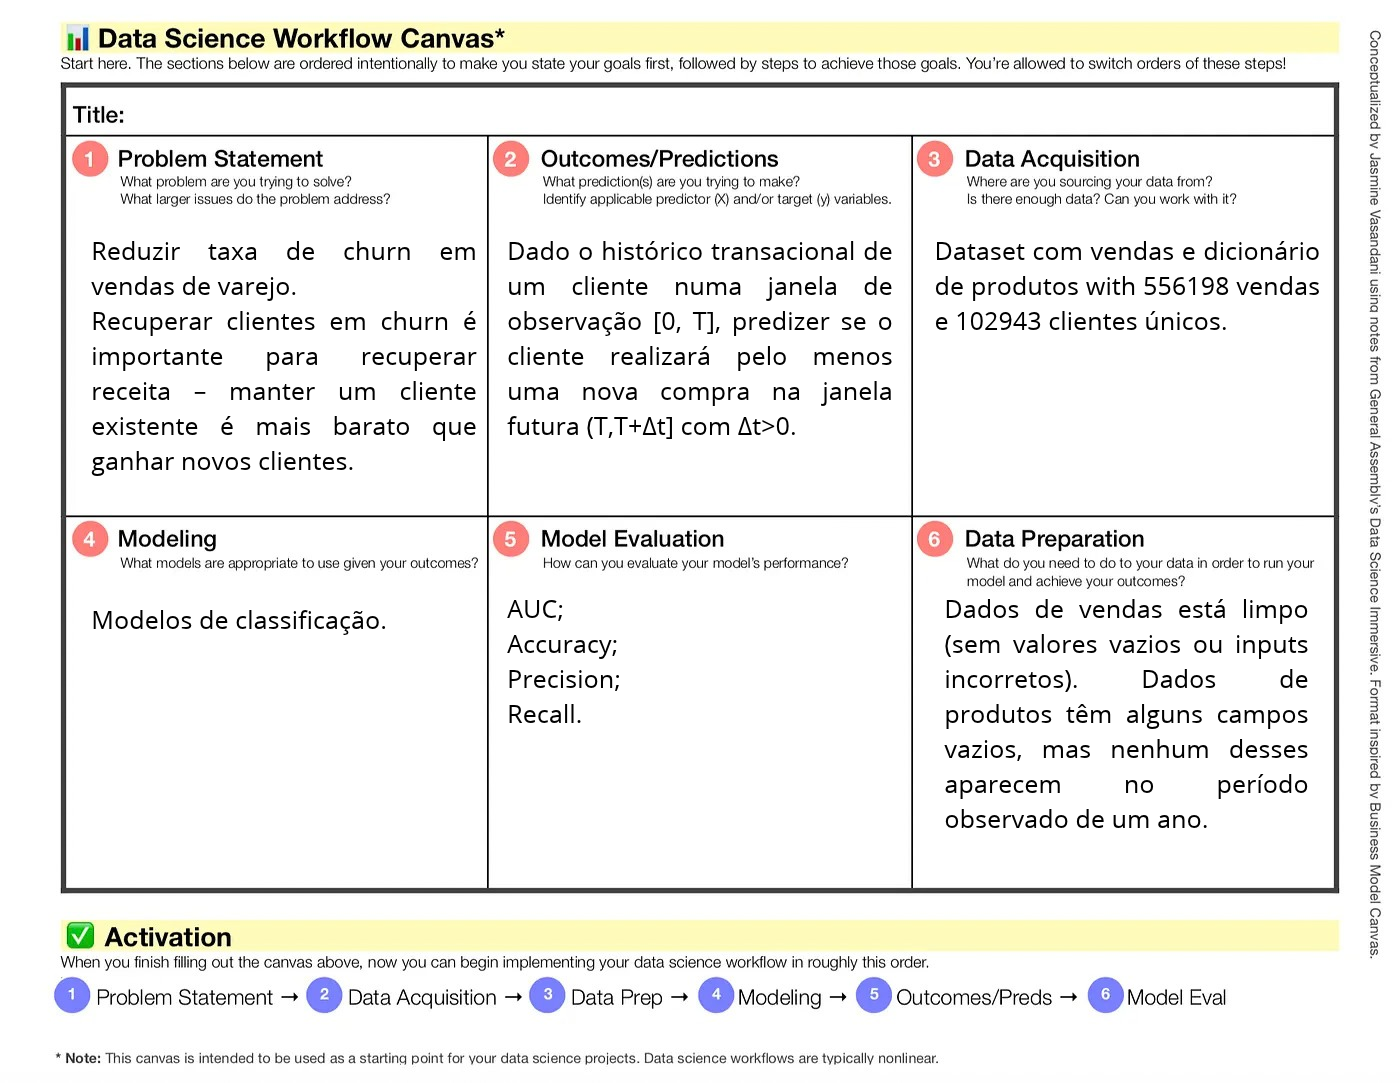
\includegraphics[width=0.95\linewidth, height=0.60\textheight, keepaspectratio]{../latex/imagens/canva2.png}}
    \end{column}
  \end{columns}
\end{frame}

% ==============================================================================
% SEÇÃO 2: DADOS, QUALIDADE E INSIGHTS DA EDA
% ==============================================================================
\section{2. Dados e Insights da EDA}

% SLIDE 3: Qualidade, LGPD e Granularidade
\begin{frame}{Qualidade, LGPD e Granularidade}
  \framesubtitle{Preparação da base transacional antes da engenharia de atributos}
  \begin{columns}[T]
    \begin{column}{0.31\textwidth}
      \card[AccentTeal]{\linewidth}{%
        {\normalsize\bfseries\color{AccentTeal}1. Integridade}\\[0.15cm]
        \footnotesize\textbf{100\% de preenchimento} nos \textbf{556.198} registros de vendas e nos \textbf{59 SKUs} ativos em 2024.\\[0.12cm]
        Nenhum campo nulo ou inconsistente no período analisado.
      }
    \end{column}
    \begin{column}{0.31\textwidth}
      \card[PoliBlue]{\linewidth}{%
        {\normalsize\bfseries\color{PoliBlue}2. Privacidade (LGPD)}\\[0.15cm]
        \footnotesize\texttt{CLI\_CPF} pseudonimizado por \textbf{\textit{hash} irreversível} na origem.\\[0.12cm]
        Identificador removido antes da etapa de treinamento dos modelos.
      }
    \end{column}
    \begin{column}{0.33\textwidth}
      \card[WarnAmber]{\linewidth}{%
        {\normalsize\bfseries\color{WarnAmber}3. Granularidade}\\[0.15cm]
        \footnotesize De item faturado para \textbf{visita diária por cliente} (\texttt{CLI\_CPF} + \texttt{DATA\_ATEND}).\\[0.12cm]
        \textbf{297.257 visitas únicas} consolidadas.
      }
    \end{column}
  \end{columns}

  \vspace{0.25cm}
  \begin{center}
    \card[NavyDark]{0.94\textwidth}{%
      \footnotesize\textbf{Por que consolidar por visita diária?} Evita distorcer a métrica de frequência quando um cliente adquire múltiplos itens no mesmo cupom fiscal.
    }
  \end{center}
\end{frame}

% SLIDE 4: Definição Empírica do Churn (Janela de 90 Dias)
\begin{frame}{Definição Empírica do \textit{Churn} (Janela de 90 Dias)}
  \framesubtitle{Critério fundamentado pela distribuição dos intervalos de recompra}
  \begin{columns}[T]
    \begin{column}{0.44\textwidth}
      \card[PoliBlue]{\linewidth}{%
        \footnotesize\textbf{Perfil da Base (102.943 clientes):}
        \begin{itemize}\setlength{\itemsep}{2pt}
          \item \textbf{50,20\%} \textit{one-timers} (51.678 clientes)
          \item \textbf{49,80\%} recorrentes (51.265 clientes)
        \end{itemize}
      }\\[0.2cm]
      \card[AlertCoral]{\linewidth}{%
        \footnotesize\textbf{\color{AlertCoral}Critério Oficial (\texttt{flag\_churn}):}\\[0.08cm]
        \textbf{90 dias (3 meses)} sem compra caracterizam evasão.\\[0.08cm]
        Janela não arbitrária: cobre \textbf{83,88\%} de todas as recompras observadas.
      }
    \end{column}
    \begin{column}{0.54\textwidth}
      \card[AccentTeal]{\linewidth}{%
        \footnotesize\textbf{Ciclo de Recompra ($N = 194.314$ intervalos):}\\[0.18cm]
        \centering
        \scriptsize
        \resizebox{\linewidth}{!}{%
        \begin{tabular}{lrrr}
          \toprule
          \textbf{Percentil} & \textbf{Q1 (25\%)} & \textbf{Mediana (50\%)} & \textbf{Q3 (75\%)} \\
          \midrule
          \textbf{Intervalo} & \textbf{14 dias} & \textbf{29 dias} & \textbf{63 dias} \\
          \bottomrule
        \end{tabular}%
        }
        \vspace{0.28cm}

        \begin{tikzpicture}[scale=0.82]
          \draw[BorderGray, line width=5pt, line cap=round] (0,0) -- (6.2,0);
          \draw[AccentTeal, line width=5pt, line cap=round] (0,0) -- (5.2,0);
          \foreach \x/\lbl/\val in {0.8/Q1/14d, 1.8/Mediana/29d, 3.8/Q3/63d, 5.2/Corte/90d} {
            \fill[NavyDark] (\x,0) circle (2.8pt);
            \node[above=4pt, font=\scriptsize\bfseries] at (\x,0) {\val};
            \node[below=4pt, font=\tiny\color{TextMuted}] at (\x,0) {\lbl};
          }
          \node[anchor=west, font=\scriptsize\bfseries\color{AccentTeal}] at (5.35, 0.0) {83,88\%};
        \end{tikzpicture}
      }
    \end{column}
  \end{columns}
\end{frame}

% SLIDE 5: Síntese das Hipóteses Exploratórias
\begin{frame}{Síntese das Hipóteses Exploratórias}
  \framesubtitle{Principais achados da Análise Exploratória de Dados (EDA) e impacto na modelagem}
  \centering
  \footnotesize
  \renewcommand{\arraystretch}{1.28}
  \resizebox{\textwidth}{!}{%
  \begin{tabular}{p{2.9cm}p{3.6cm}cp{5.7cm}}
    \toprule
    \textbf{Hipótese} & \textbf{Enunciado} & \textbf{Veredito} & \textbf{Evidência Numérica Principal} \\
    \midrule
    \textbf{H1:} Passagem vs. Desengajados & Coexistência de compra única e recorrentes no \textit{churn}. & \cellcolor{AccentTeal!15}\textbf{\color{AccentTeal}Confirmada} & \textbf{66,93\%} de todo o \textit{churn} vem de \textit{one-timers} (falha na conversão para a 2ª compra). \\
    \textbf{H2.1:} Aumento do Intervalo & Intervalo entre compras aumenta antes do \textit{churn}. & \cellcolor{AlertCoral!15}\textbf{\color{AlertCoral}Refutada} & Medianas praticamente idênticas: $33 \rightarrow 34 \rightarrow 36$d (ativos) vs. $31 \rightarrow 32 \rightarrow 36$d (evadidos). \\
    \textbf{H2.2:} Categorias de Rotina & Itens de rotina doméstica retêm mais que consumo imediato. & \cellcolor{AccentTeal!15}\textbf{\color{AccentTeal}Confirmada} & Recorrência em \textit{Conservas} (\textbf{76,0\%}) e \textit{Matinais} (\textbf{74,4\%}) vs. \textit{Lanchonete} (\textbf{49,0\%} de \textit{churn}). \\
    \textbf{H3:} Tipo de Filial & Canal (\texttt{SHOPPING} vs. \texttt{RUA}) influencia retenção. & \cellcolor{AccentTeal!15}\textbf{\color{AccentTeal}Confirmada} & Clientes \textbf{híbridos} têm apenas \textbf{33,41\%} de \textit{churn} (vs. 55,40\% Shopping e 52,07\% Rua). \\
    \bottomrule
  \end{tabular}%
  }
\end{frame}

% ==============================================================================
% SEÇÃO 3: ARQUITETURA DO PROJETO E MODELAGEM
% ==============================================================================
\section{3. Arquitetura e Modelagem}

% SLIDE 6: Arquitetura de Dados em Camadas (SQLite)
\begin{frame}{Arquitetura de Dados em Camadas (SQLite)}
  \framesubtitle{Separação entre dados brutos, \textit{feature store} e tabela analítica de treino}
  \begin{columns}[c]
    \begin{column}{0.44\textwidth}
      \footnotesize\textbf{Banco relacional (\texttt{banco\_de\_dados.db})} em 3 camadas:\\[0.12cm]
      \card[PoliBlue]{\linewidth}{%
        \scriptsize\textbf{1. Camada Bruta:}\\
        \texttt{vendas} e \texttt{produto} — imutáveis, fonte única da verdade.
      }\\[0.1cm]
      \card[AccentTeal]{\linewidth}{%
        \scriptsize\textbf{2. Camada de Atributos (\texttt{tb\_book}):}\\
        \textbf{32 variáveis} comportamentais agregadas por cliente em cada \texttt{dt\_ref}.
      }\\[0.1cm]
      \card[NavyDark]{\linewidth}{%
        \scriptsize\textbf{3. Camada Analítica (\texttt{tb\_abt\_churn}):}\\
        Cruzamento de \texttt{tb\_book} com o comportamento futuro (\texttt{flag\_churn}).
      }
    \end{column}
    \begin{column}{0.54\textwidth}
      \centering
      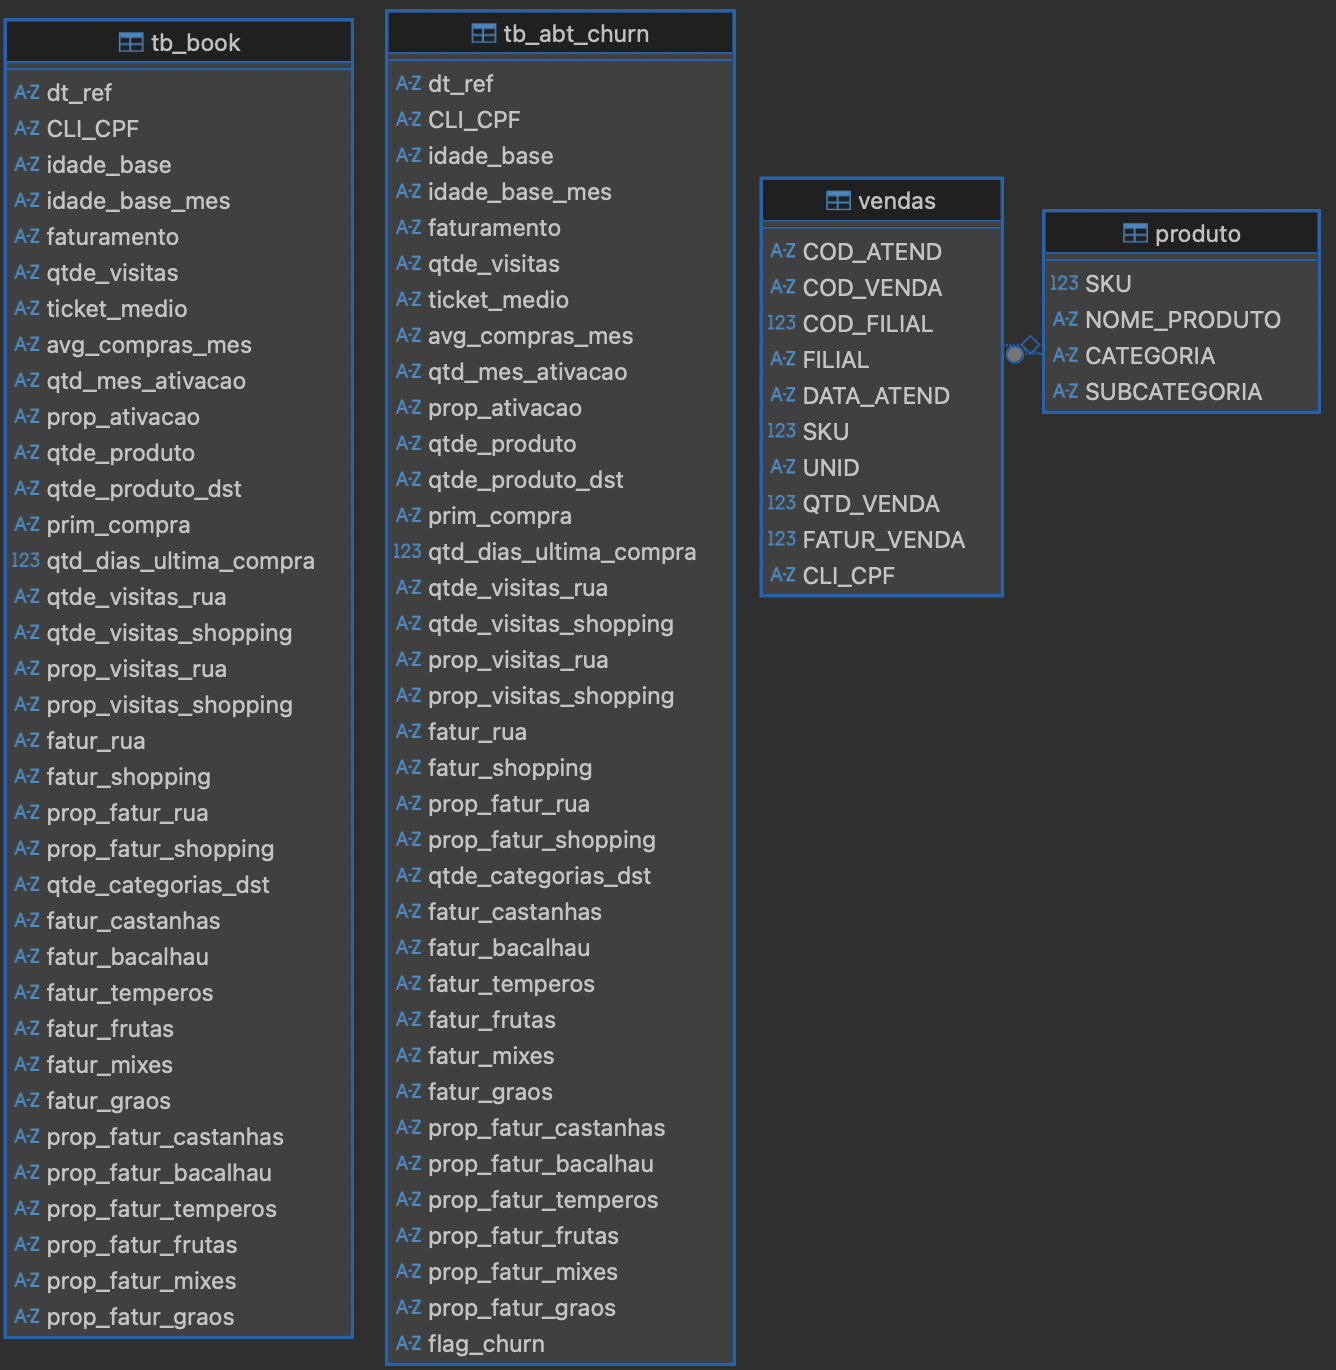
\includegraphics[width=\linewidth, height=0.58\textheight, keepaspectratio]{../latex/imagens/diagrama_db_2.png}
    \end{column}
  \end{columns}
\end{frame}

% SLIDE 7: Pipeline Modular e Reprodutível
\begin{frame}{Pipeline Modular e Reprodutível}
  \framesubtitle{Arquitetura inspirada na série DTona, dividida em 4 scripts sequenciais}
  \vspace{0.1cm}
  \begin{center}
    \begin{tikzpicture}[
      stepbox/.style={draw=PoliBlue, fill=SoftBg, rounded corners=5pt, text width=2.75cm, minimum height=2.45cm, align=center, inner sep=5pt, line width=1pt},
      arrow/.style={-{Stealth[length=2.8mm]}, thick, NavyDark}
    ]
      \node[stepbox] (s1) {
        \footnotesize\textbf{\color{PoliBlue}1. Safra / Book}\\[0.1cm]
        \scriptsize\texttt{queries/}\\\texttt{exec\_safra.py}\\
        (\texttt{features.sql})\\[0.1cm]
        Popula \texttt{tb\_book} com \textbf{idempotência} (\texttt{DELETE}+\texttt{INSERT}).
      };
      \node[stepbox, right=0.45cm of s1] (s2) {
        \footnotesize\textbf{\color{PoliBlue}2. Montagem ABT}\\[0.1cm]
        \scriptsize\texttt{data\_prep/train/}\\\texttt{exec\_abt.py}\\
        (\texttt{abt.sql})\\[0.1cm]
        Gera \texttt{tb\_abt\_churn} com o alvo futuro.
      };
      \node[stepbox, right=0.45cm of s2] (s3) {
        \footnotesize\textbf{\color{PoliBlue}3. Treinamento}\\[0.1cm]
        \scriptsize\texttt{modelling/train/}\\\texttt{model.py}\\
        (\texttt{random\_state=2026})\\[0.1cm]
        Treina 7 modelos e salva \texttt{best\_model.pkl}.
      };
      \node[stepbox, right=0.45cm of s3, draw=AccentTeal] (s4) {
        \footnotesize\textbf{\color{AccentTeal}4. Predição}\\[0.1cm]
        \scriptsize\texttt{modelling/predict/}\\\texttt{predict.py}\\[0.2cm]
        Escora a safra de produção (\texttt{2025-01-01}).
      };

      \draw[arrow] (s1) -- (s2);
      \draw[arrow] (s2) -- (s3);
      \draw[arrow] (s3) -- (s4);
    \end{tikzpicture}
  \end{center}

  \vspace{0.2cm}
  \begin{center}
    \card[AccentTeal]{0.95\textwidth}{%
      \footnotesize\textbf{Destaques de Engenharia:} Reprodutibilidade garantida (\texttt{random\_state=2026}), automação completa e \textbf{idempotência} — reprocessar uma safra não gera duplicatas.
    }
  \end{center}
\end{frame}

% SLIDE 8: Engenharia de Atributos e Prevenção de Data Leakage
\begin{frame}{Engenharia de Atributos e Prevenção de \textit{Data Leakage}}
  \framesubtitle{Isolamento temporal estrito entre janela de observação e janela de maturação}
  \begin{center}
    \begin{tikzpicture}
      \fill[PoliBlue!15, rounded corners=3pt] (0,0) rectangle (7.2,0.88);
      \fill[AlertCoral!15, rounded corners=3pt] (7.4,0) rectangle (13.2,0.88);
      \draw[NavyDark, thick] (7.3,-0.1) -- (7.3,0.98);
      \node[font=\scriptsize\color{PoliBlue}, align=center] at (3.6, 0.44) {\textbf{Janela de Observação (6 meses)}\\$[\texttt{dt\_ref}-6\text{m}, \; \texttt{dt\_ref}) \rightarrow$ \textbf{32 features}};
      \node[font=\scriptsize\color{AlertCoral}, align=center] at (10.3, 0.44) {\textbf{Janela de Maturação / Target (3 meses)}\\$[\texttt{dt\_ref}, \; \texttt{dt\_ref}+3\text{m}) \rightarrow$ \texttt{flag\_churn}};
      \node[above=1pt, font=\scriptsize\bfseries\color{NavyDark}] at (7.3, 0.96) {\texttt{dt\_ref}};
    \end{tikzpicture}
  \end{center}

  \vspace{0.05cm}
  \centering
  \scriptsize
  \renewcommand{\arraystretch}{1.12}
  \resizebox{\textwidth}{!}{%
  \begin{tabular}{p{3.4cm}p{9.8cm}}
    \toprule
    \textbf{Dimensão (32 Features)} & \textbf{Principais Atributos} \\
    \midrule
    1. Relacionamento e Recência & \texttt{idade\_base}, \texttt{idade\_base\_mes}, \texttt{qtd\_dias\_ultima\_compra} \\
    2. Frequência e Regularidade & \texttt{qtde\_visitas}, \texttt{avg\_compras\_mes}, \texttt{qtd\_mes\_ativacao}, \texttt{prop\_ativacao} \\
    3. Monetário e Volume & \texttt{faturamento}, \texttt{ticket\_medio}, \texttt{qtde\_produto}, \texttt{qtde\_produto\_dst} \\
    4. Canal (Rua vs. Shopping) & \texttt{qtde\_visitas\_rua}, \texttt{qtde\_visitas\_shopping}, \texttt{prop\_visitas\_*}, \texttt{fatur\_*}, \texttt{prop\_fatur\_*} \\
    5. Mix de Categorias & \texttt{qtde\_categorias\_dst}, \texttt{fatur\_[cat]}, \texttt{prop\_fatur\_[cat]} (6 categorias = $>80\%$ da receita) \\
    \bottomrule
  \end{tabular}%
  }

  \vspace{0.08cm}
  \noindent\parbox{\textwidth}{\scriptsize\textbf{\color{AlertCoral}Segurança:} \texttt{CLI\_CPF}, \texttt{dt\_ref} e \texttt{prim\_compra} removidos do treino para evitar vazamento e dependência de calendário.}
\end{frame}

% SLIDE 9: Safras, Validação Temporal (Out-Of-Time) e Modelos
\begin{frame}{Safras, Validação Temporal (\textit{Out-Of-Time}) e Modelos}
  \framesubtitle{4 safras maturadas (271.783 registros) + safra de produção 2025 + 7 algoritmos}
  \centering
  \scriptsize
  \renewcommand{\arraystretch}{1.28}
  \begin{tabular}{llllrr}
    \toprule
    \textbf{Safra (\texttt{dt\_ref})} & \textbf{Janela Atributos (6m)} & \textbf{Janela Target (3m)} & \textbf{Finalidade} & \textbf{Clientes} & \textbf{Taxa \textit{Churn}} \\
    \midrule
    \texttt{2024-07-01} & 01/01/24 a 30/06/24 & 01/07/24 a 30/09/24 & Desenvolvimento (80/20) & 65.356 & 59,06\% \\
    \texttt{2024-08-01} & 01/02/24 a 31/07/24 & 01/08/24 a 31/10/24 & Desenvolvimento (80/20) & 67.186 & 59,49\% \\
    \texttt{2024-09-01} & 01/03/24 a 31/08/24 & 01/09/24 a 30/11/24 & Desenvolvimento (80/20) & 69.540 & 60,74\% \\
    \rowcolor{PoliBlue!10}
    \texttt{2024-10-01} & 01/04/24 a 30/09/24 & 01/10/24 a 31/12/24 & \textbf{Validação OOT} & \textbf{69.701} & \textbf{59,78\%} \\
    \midrule
    \rowcolor{AccentTeal!12}
    \texttt{2025-01-01} & 01/07/24 a 31/12/24 & 01/01/25 a 31/03/25* & \textbf{Predição Produção} & \textbf{73.101} & \textit{A prever} \\
    \bottomrule
  \end{tabular}

  \vspace{0.3cm}
  \begin{columns}[T]
    \begin{column}{0.48\textwidth}
      \card[PoliBlue]{\linewidth}{%
        \textbf{Divisão Temporal:}
        \begin{itemize}\setlength{\itemsep}{2pt}
          \item \textbf{Desenvolvimento:} 202.082 reg. (80\% Treino / 20\% Teste \textit{In-Time})
          \item \textbf{Validação OOT:} Out/2024 inteira (69.701 reg.) simulando produção futura.
        \end{itemize}
      }
    \end{column}
    \begin{column}{0.48\textwidth}
      \card[AccentTeal]{\linewidth}{%
        \textbf{7 Algoritmos Testados:}
        \footnotesize Árvore sem Poda (ref. \textit{overfitting}), Árvore com Poda, Regressão Logística, SVM Linear, \textbf{Random Forest}, Gradient Boosting (HistGB) e Rede Neural (MLP).
      }
    \end{column}
  \end{columns}
\end{frame}

% ==============================================================================
% SEÇÃO 4: RESULTADOS E PREDIÇÃO PARA 2025
% ==============================================================================
\section{4. Resultados e Predição 2025}

% SLIDE 10: Comparativo de Desempenho dos Modelos (OOT)
\begin{frame}{Comparativo de Desempenho dos Modelos (OOT)}
  \framesubtitle{Critério principal: ROC AUC na base OOT (capacidade de ordenação por risco)}
  \centering
  \scriptsize
  \renewcommand{\arraystretch}{1.22}
  \resizebox{\textwidth}{!}{%
  \begin{tabular}{lrrrrrrrr}
    \toprule
    \textbf{Modelo} & \textbf{Acc Treino} & \textbf{Acc Teste} & \textbf{Acc OOT} & \textbf{AUC Treino} & \textbf{AUC Teste} & \textbf{AUC OOT} & \textbf{F1 Teste} & \textbf{F1 OOT} \\
    \midrule
    \rowcolor{AccentTeal!15}
    \textbf{Random Forest (Escolhido)} & 0,7263 & \textbf{0,7210} & 0,7205 & 0,7630 & 0,7541 & \textbf{0,7620} & \textbf{0,7888} & \textbf{0,7828} \\
    Gradient Boosting (HistGB) & 0,7238 & 0,7209 & \textbf{0,7209} & 0,7607 & \textbf{0,7545} & \textbf{0,7620} & 0,7882 & 0,7823 \\
    Rede Neural (MLP) & 0,7187 & 0,7177 & 0,7181 & 0,7523 & 0,7508 & 0,7594 & 0,7862 & 0,7787 \\
    Regressão Logística & 0,7142 & 0,7157 & 0,7164 & 0,7460 & 0,7479 & 0,7573 & 0,7862 & 0,7794 \\
    SVM Linear & 0,7127 & 0,7145 & 0,7141 & 0,7454 & 0,7473 & 0,7571 & 0,7840 & 0,7750 \\
    Decision Tree (Com Poda) & 0,7330 & 0,7098 & 0,7064 & 0,7757 & 0,7371 & 0,7442 & 0,7762 & 0,7684 \\
    \rowcolor{AlertCoral!12}
    Decision Tree (Sem Poda) & \textbf{0,9940} & 0,6404 & 0,6313 & \textbf{0,9999} & 0,6285 & 0,6208 & 0,6983 & 0,6881 \\
    \bottomrule
  \end{tabular}%
  }

  \vspace{0.25cm}
  \begin{columns}[T]
    \begin{column}{0.48\textwidth}
      \card[AccentTeal]{\linewidth}{%
        \footnotesize\textbf{Por que Random Forest?} Empate no AUC OOT (\textbf{0,7620}) com HistGB, mas \textbf{F1-Score superior} no Teste (0,7888) e no OOT (0,7828).
      }
    \end{column}
    \begin{column}{0.48\textwidth}
      \card[AlertCoral]{\linewidth}{%
        \footnotesize\textbf{Contraste de Generalização:} Árvore sem poda memorizou o treino (AUC \textbf{0,9999}) e despencou no OOT (\textbf{0,6208}) — \textit{overfitting} severo.
      }
    \end{column}
  \end{columns}
\end{frame}

% SLIDE 11: O que Explica o Churn? (Feature Importance e Correlação)
\begin{frame}{O que Explica o \textit{Churn}? (\textit{Feature Importance} e Correlação)}
  \framesubtitle{12 variáveis concentram 90,68\% da capacidade preditiva do Random Forest}
  \begin{columns}[c]
    \begin{column}{0.53\textwidth}
      \scriptsize
      \renewcommand{\arraystretch}{1.04}
      \begin{tabular}{rlrr}
        \toprule
        \textbf{Pos.} & \textbf{Variável Explicativa} & \textbf{Imp. (\%)} & \textbf{Acum. (\%)} \\
        \midrule
        1º & \texttt{qtde\_visitas} & \textbf{22,02\%} & 22,02\% \\
        2º & \texttt{qtd\_mes\_ativacao} & \textbf{19,33\%} & \textbf{41,35\%} \\
        3º & \texttt{qtde\_produto} & 11,33\% & 52,68\% \\
        4º & \texttt{qtde\_produto\_dst} & 5,78\% & 58,46\% \\
        5º & \texttt{qtde\_visitas\_rua} & 5,38\% & 63,84\% \\
        6º & \texttt{qtde\_categorias\_dst} & 4,85\% & 68,69\% \\
        7º & \texttt{qtde\_visitas\_shopping} & 4,68\% & 73,36\% \\
        8º & \texttt{prop\_ativacao} & 3,81\% & 77,17\% \\
        9º & \texttt{qtd\_dias\_ultima\_compra} & 3,71\% & 80,88\% \\
        10º & \texttt{idade\_base\_mes} & 3,60\% & 84,48\% \\
        \bottomrule
      \end{tabular}
    \end{column}
    \begin{column}{0.45\textwidth}
      \card[PoliBlue]{\linewidth}{%
        \scriptsize\textbf{Frequência + Regularidade = 41,35\%}: \texttt{qtde\_visitas} (22,02\%) e \texttt{qtd\_mes\_ativacao} (19,33\%) dominam a decisão do modelo.
      }\\[0.08cm]
      \card[AccentTeal]{\linewidth}{%
        \scriptsize\textbf{Hábito vs. Categoria Isolada:} Variedade da cesta pesa mais que categorias isoladas (12 vars de categoria = \textbf{4,06\%}).
      }\\[0.08cm]
      \card[WarnAmber]{\linewidth}{%
        \scriptsize\textbf{Multicolinearidade:} \textbf{14 pares} com $|r| \ge 0,80$ (ex.: proporções Rua/Shopping) mapeados para simplificação futura.
      }
    \end{column}
  \end{columns}
\end{frame}

% SLIDE 12: Predição de Produção — Safra 2025-01-01
\begin{frame}{Predição de Produção — Safra \texttt{2025-01-01}}
  \framesubtitle{Escoragem dos clientes ativos do 2º sem/2024 para o 1º trimestre de 2025}
  \begin{columns}[T]
    \begin{column}{0.32\textwidth}
      \kpicard[PoliBlue]{\linewidth}{73.101}\\[-0.08cm]
      \centering\scriptsize\textbf{Clientes Ativos} (R\$ 4,67M no 2º sem/24)
    \end{column}
    \begin{column}{0.32\textwidth}
      \kpicard[AlertCoral]{\linewidth}{66,90\%}\\[-0.08cm]
      \centering\scriptsize\textbf{Em Risco ($p \ge 0,50$)} (48.908 clientes)
    \end{column}
    \begin{column}{0.32\textwidth}
      \kpicard[WarnAmber]{\linewidth}{56,76\%}\\[-0.08cm]
      \centering\scriptsize\textbf{Probabilidade Média} de \textit{Churn}
    \end{column}
  \end{columns}

  \vspace{0.25cm}
  \centering
  \scriptsize
  \renewcommand{\arraystretch}{1.3}
  \resizebox{\textwidth}{!}{%
  \begin{tabular}{lrrrrrl}
    \toprule
    \textbf{Faixa de Risco} & \textbf{Clientes} & \textbf{\% Base} & \textbf{Prob. Média} & \textbf{Faturamento 6m} & \textbf{Recência} & \textbf{Ação Recomendada} \\
    \midrule
    \textbf{\color{AccentTeal}1. Baixo ($<40\%$)} & 16.041 & 21,94\% & 22,76\% & \textbf{R\$ 2,29 mi} & 32,0d & Manter sem descontos agressivos \\
    \textbf{\color{WarnAmber}2. Médio ($40\%$--$70\%$)} & 30.153 & 41,25\% & 56,19\% & \textbf{R\$ 1,45 mi} & 75,8d & Foco de campanhas preventivas \\
    \textbf{\color{AlertCoral}3. Alto ($\ge 70\%$)} & 26.907 & 36,81\% & 77,66\% & \textbf{R\$ 925,77 mil} & 92,7d & Ações diretas de reativação \\
    \midrule
    \textbf{Total / Geral} & \textbf{73.101} & \textbf{100,00\%} & \textbf{56,76\%} & \textbf{R\$ 4,67 mi} & \textbf{72,4d} & Priorização de orçamento \\
    \bottomrule
  \end{tabular}%
  }
\end{frame}

% SLIDE 13: Priorização — Top VIPs em Alto Risco
\begin{frame}{Priorização — Top VIPs em Alto Risco}
  \framesubtitle{Cruzamento Risco ($\ge 70\%$) $\times$ Faturamento 6m para ação comercial imediata}
  \begin{columns}[T]
    \begin{column}{0.63\textwidth}
      \centering
      \scriptsize
      \renewcommand{\arraystretch}{1.15}
      \resizebox{\linewidth}{!}{%
      \begin{tabular}{lrrrrr}
        \toprule
        \textbf{Cliente (\texttt{CLI\_CPF})} & \textbf{Prob.} & \textbf{Fat. 6m (R\$)} & \textbf{Visitas} & \textbf{Ticket (R\$)} & \textbf{Rec. (d)} \\
        \midrule
        \texttt{45b38f904157} & 79,96\% & 1.201,60 & 1 & 1.201,60 & 11 \\
        \texttt{10132655ccfa} & 78,57\% & 1.081,29 & 1 & 1.081,29 & 16 \\
        \texttt{56df144b2e93} & 76,05\% &   931,85 & 1 &   931,85 & 24 \\
        \texttt{d3ca26b61b5b} & 79,20\% &   913,53 & 1 &   913,53 & 13 \\
        \texttt{723abe558371} & 85,14\% &   880,72 & 1 &   880,72 & 51 \\
        \texttt{91531c44c498} & 80,46\% &   814,98 & 1 &   814,98 & 76 \\
        \texttt{bba3a36b6a36} & 84,19\% &   784,28 & 1 &   784,28 & 39 \\
        \texttt{1d26cf9ff26b} & 76,89\% &   779,59 & 1 &   779,59 & 34 \\
        \texttt{d60700adf30a} & 79,82\% &   735,92 & 1 &   735,92 & 15 \\
        \texttt{26fe8365dea9} & 81,26\% &   717,84 & 1 &   717,84 & 28 \\
        \bottomrule
      \end{tabular}%
      }
    \end{column}
    \begin{column}{0.35\textwidth}
      \card[AlertCoral]{\linewidth}{%
        \footnotesize\textbf{\color{AlertCoral}Padrão Comum:}\\[0.1cm]
        Todos os Top 10 faturaram entre \textbf{R\$ 717,84 e R\$ 1.201,60}, mas realizaram \textbf{apenas 1 visita} no semestre (\textit{one-timers} de alto ticket).
      }\\[0.22cm]
      \card[AccentTeal]{\linewidth}{%
        \footnotesize\textbf{\color{AccentTeal}Ação Imediata:}\\[0.1cm]
        Abordagem personalizada para conversão da \textbf{2ª compra} antes que completem \textbf{90 dias}.
      }
    \end{column}
  \end{columns}
\end{frame}

% ==============================================================================
% SEÇÃO 5: CONCLUSÃO E PRÓXIMOS PASSOS
% ==============================================================================
\section{5. Conclusão e Próximos Passos}

% SLIDE 14: Conclusão e Próximos Passos
\begin{frame}{Conclusão e Próximos Passos}
  \framesubtitle{Síntese de valor entregue e evolução recomendada}
  \begin{columns}[T]
    \begin{column}{0.44\textwidth}
      \card[AccentTeal]{\linewidth}{%
        {\normalsize\bfseries\color{AccentTeal}Entrega Principal}\\[0.18cm]
        \footnotesize\textit{Pipeline} ponta a ponta \textbf{reprodutível}, sem vazamento temporal, validado em OOT (\textbf{ROC AUC 0,7620}) e pronto para operação.\\[0.2cm]
        Lista priorizada gerada pelo \texttt{predict.py} já permite segmentar orçamento de retenção por faixa de risco e valor.
      }
    \end{column}
    \begin{column}{0.52\textwidth}
      \card[PoliBlue]{\linewidth}{%
        {\normalsize\bfseries\color{PoliBlue}Próximos Passos}\\[0.18cm]
        \footnotesize
        \begin{enumerate}\setlength{\itemsep}{4pt}
          \item \textbf{Acompanhamento Real e Testes A/B:} Monitorar a safra \texttt{2025-01-01} e testar campanhas de retenção por faixa de risco.
          \item \textbf{Redução de Dimensionalidade:} Remover variáveis redundantes ($|r| \ge 0,80$) mapeadas na análise de multicolinearidade.
          \item \textbf{Análise de Sobrevivência:} Prever \textit{quando} o cliente evade, complementando a classificação binária.
        \end{enumerate}
      }
    \end{column}
  \end{columns}

  \vspace{0.3cm}
  \begin{center}
    {\large\bfseries\color{NavyDark}Obrigado! \quad Perguntas?}
  \end{center}
\end{frame}

\end{document}
